% !TEX root = ../algorithms.tex

\section{Приближённые алгоритмы}

Многие важные задачи оптимизации являются NP-полными: для них неизвестно полиномиальных алгоритмов, а нахождение точного ответа, по всей видимости, требует экспоненциального времени. На практике такие задачи обычно решаются либо эвристиками (без гарантий качества), либо \emph{приближёнными алгоритмами} — полиномиальными методами, гарантирующими ответ, близкий к оптимальному.

\begin{Definition}{Приближённый алгоритм ($\rho$-приближение)}{}
	Пусть дана задача оптимизации $f\colon \mathrm{input} \to \mathbb{R}$, решаемая на максимум или минимум. Для $\rho \geq 1$ алгоритм $g$ называется \emph{$\rho$-приближением}, если для любого входа $x$:
	\begin{align*}
		g(x) &\geq \frac{f^*(x)}{\rho} \quad \text{(для задачи максимизации),} \\
		g(x) &\leq f^*(x) \cdot \rho \quad \text{(для задачи минимизации),}
	\end{align*}
	где $f^*(x)$ — оптимальное значение на входе $x$.
\end{Definition}

\begin{Remark}{}{}
	Величина $\rho$ называется \emph{коэффициентом приближения} (approximation ratio). Чем меньше $\rho$, тем лучше алгоритм. Значение $\rho = 1$ соответствует точному решению.
\end{Remark}

\subsection{Задача о вершинном покрытии}

\begin{Definition}{Вершинное покрытие}{}
	Дан граф $G = (V, E)$. \emph{Вершинное покрытие} — это подмножество $C \subseteq V$ такое, что для каждого ребра $e \in E$ хотя бы один из его концов принадлежит $C$:
	\[
	\forall \{u,v\} \in E \;\; \exists\, w \in C \colon w \in \{u,v\}.
	\]
\end{Definition}

\textbf{Задача:} найти вершинное покрытие минимального размера $|C|$.

Задача о вершинном покрытии является NP-полной. Для неё неизвестно полиномиальных алгоритмов (в стандартной теории $\mathrm{P} \neq \mathrm{NP}$). Однако существует простой 2-приближённый алгоритм, основанный на жадном построении паросочетания.

\subsubsection*{Алгоритм жадного паросочетания}

\textbf{Алгоритм (2-приближённый для задачи о вершинном покрытии):}
\begin{enumerate}
	\item Выбрать произвольное ребро $\{u,v\} \in E$.
	\item Добавить обе вершины в покрытие: $C \coloneqq C \cup \{u, v\}$.
	\item Удалить из графа $u$, $v$ и все инцидентные им рёбра: $G \coloneqq G \setminus \{u,v\}$.
	\item Если $E(G) \neq \varnothing$, перейти к шагу~1.
\end{enumerate}

\medskip

На выходе $C$ является вершинным покрытием, поскольку каждое ребро было <<обработано>> на некотором шаге.

\begin{Statement}{Алгоритм жадного паросочетания даёт 2-приближение}{}
	Пусть $C^*$ — минимальное вершинное покрытие. Тогда $|C| \leq 2\,|C^*|$.
\end{Statement}

\begin{proof}
В ходе алгоритма строится набор рёбер $M$ (паросочетание): на каждом шаге выбирается ребро $\{u,v\}$, причём после удаления $u$ и $v$ ни одно из последующих рёбер не касается $u$ или $v$. Таким образом, $M$ — паросочетание размера $|C|/2$.

Так как $C^*$ является вершинным покрытием, каждое ребро из $M$ должно иметь хотя бы один конец в $C^*$. Поскольку рёбра паросочетания не делят вершин, различным рёбрам из $M$ соответствуют различные вершины из $C^*$. Следовательно,
\[
|C^*| \geq |M| = \frac{|C|}{2} \implies |C| \leq 2\,|C^*|. 
\]
\end{proof}

\subsection{Задача о взвешенном вершинном покрытии}

Дан граф $G=(V,E)$ и функция весов $w\colon V \to \mathbb{R}_{>0}$. Требуется найти вершинное покрытие $C\subseteq V$ минимального суммарного веса:
\[
\sum_{v \in C} w(v) \to \min.
\]

Алгоритм жадного паросочетания в этом случае \emph{не работает} с прежней гарантией, поскольку не учитывает веса вершин. Задача о взвешенном вершинном покрытии также NP-полная (эквивалентна по трудности невзвешенному случаю).

\subsubsection*{Сведение к целочисленному линейному программированию}

Введём переменные $x_v \in \{0,1\}$ для каждой вершины $v$: $x_v = 1$ означает, что вершина $v$ включена в покрытие. Задача записывается как:
\[
\begin{cases}
	\displaystyle\min_{x} \sum_{v \in V} w(v)\cdot x_v, \\[4pt]
	x_u + x_v \geq 1 \quad \forall\, \{u,v\} \in E, \\[2pt]
	0 \leq x_v \leq 1 \quad \forall\, v \in V, \\[2pt]
	x_v \in \{0,1\}.
\end{cases}
\]

\subsubsection*{2-приближённый алгоритм через LP-релаксацию}

Снимем условие целочисленности и решим непрерывную \emph{LP-релаксацию} (без ограничения $x_v \in \{0,1\}$):
\[
\begin{cases}
	\displaystyle\min \sum_{v \in V} w(v)\cdot x_v, \\[4pt]
	x_u + x_v \geq 1 \quad \forall\, \{u,v\} \in E, \\[2pt]
	0 \leq x_v \leq 1 \quad \forall\, v \in V.
\end{cases}
\]
LP-релаксация решается за полиномиальное время, и мы находим оптимальное дробное решение $\{x^*_v\}$.

Построим целочисленное решение \emph{округлением}:
\[
C = \bigl\{\, v \in V \mid x^*_v \geq \tfrac{1}{2} \,\bigr\}, \qquad
\bar{x}_v = \begin{cases} 1, & v \in C, \\ 0, & v \notin C. \end{cases}
\]

\begin{Theorem}{О 2-приближении через LP-релаксацию}{}
	Множество $C$, построенное описанным выше методом, является вершинным покрытием и 2-приближением задачи о взвешенном вершинном покрытии.
\end{Theorem}

\begin{proof}\\
\emph{Корректность покрытия.} Для каждого ребра $\{u,v\} \in E$ из ограничения LP: $x^*_u + x^*_v \geq 1$. Следовательно, хотя бы одно из двух неравенств $x^*_u \geq \tfrac{1}{2}$ или $x^*_v \geq \tfrac{1}{2}$ выполнено, то есть хотя бы одна из вершин попадает в $C$. Значит, $C$ — вершинное покрытие.

\emph{Оценка качества.} Так как $\bar{x}_v = 1$ только при $x^*_v \geq \tfrac{1}{2}$, имеем $\bar{x}_v \leq 2 x^*_v$ для всех $v$. Поэтому:
\[
\sum_{v \in V} w(v)\,\bar{x}_v \;\leq\; \sum_{v \in V} w(v) \cdot 2 x^*_v \;=\; 2\sum_{v \in V} w(v)\, x^*_v \;\leq\; 2\sum_{v \in V} w(v)\, x^{**}_v,
\]
где $\{x^{**}_v\}$ — оптимальное целочисленное решение (оно допустимо для LP, поэтому $\sum w(v) x^*_v \leq \sum w(v) x^{**}_v$). 

Следовательно, $\sum_{v \in C} w(v) \leq 2\sum_{v \in V} w(v)\,x^{**}_v$. 
\end{proof}

\begin{Remark}{}{}
	Эта задача является ещё и более оптимальной: известно, что $(2-\varepsilon)$-приближение для вершинного покрытия крайне сложно или, по-видимому, невозможно найти (при стандартных предположениях о сложности).
\end{Remark}

\subsection{Задача коммивояжёра (TSP)}

\begin{Definition}{Задача коммивояжёра (Travelling Salesman Problem)}{}
	Дан полный граф $K_n = G(V,E)$ с весами $c\colon E \to \mathbb{R}^+$ на рёбрах. Требуется найти гамильтонов цикл $H$ (цикл, проходящий через каждую вершину ровно один раз) минимального веса:
	\[
	\sum_{e \in E(H)} c(e) \to \min.
	\]
\end{Definition}

Задача о гамильтоновом цикле (даже без весов) является NP-полной, поэтому TSP — NP-полная задача. Более того, задача коммивояжёра в общем случае \emph{не имеет} хорошей приближённой аппроксимации:

\begin{Proposition}{Об иноаппроксимируемости общего TSP}{}
	Для любого $\rho \geq 1$: если существует $\rho$-приближённый полиномиальный алгоритм для задачи коммивояжёра, то существует полиномиальный алгоритм для задачи о гамильтоновом цикле (и, следовательно, $\mathrm{P} = \mathrm{NP}$).
\end{Proposition}

\begin{proof}
Пусть дан граф $\widetilde{G}(V,\widetilde{E})$, и мы хотим проверить, есть ли в нём гамильтонов цикл. Построим полный граф $K_{|V|}$ с весами:
\[
c(u,v) = \begin{cases} 1, & \{u,v\} \in \widetilde{E}, \\ M, & \{u,v\} \notin \widetilde{E}, \end{cases}
\]
где $M$ — очень большое число (например, $M = \rho\cdot|V|+1$). Запустим $\rho$-приближённый алгоритм для TSP на этом графе. Если в $\widetilde{G}$ есть гамильтонов цикл, то оптимальное решение имеет вес $|V|$, и алгоритм вернёт решение веса $\leq \rho\cdot|V| < M$. Если гамильтонова цикла нет, любой цикл использует хотя бы одно <<тяжёлое>> ребро, и его вес $\geq M > \rho\cdot|V|$. Таким образом, по ответу алгоритма можно отличить два случая.
\end{proof}

\subsection{Метрическая задача коммивояжёра}

Ситуация улучшается, если потребовать от весов выполнения \emph{неравенства треугольника}:

\begin{Definition}{Метрическая задача коммивояжёра}{}
	TSP называется \emph{метрическим}, если веса рёбер удовлетворяют неравенству треугольника:
	\[
	\forall\, u,v,w \in V \colon\quad c(u,v) + c(v,w) \geq c(u,w).
	\]
\end{Definition}

\begin{Example}{Примеры метрических весов}{}
	\begin{enumerate}
		\item $V \subseteq \mathbb{R}^2$, $c$ — евклидово расстояние (Евклидова задача коммивояжёра).
		\item $c\colon E \to \{1,2\}$ — весовая функция, принимающая только значения 1 и 2. Это тоже удовлетворяет неравенству треугольника ($1+1 \geq 1$, $1+2 \geq 2$, $2+2 \geq 2$).
	\end{enumerate}
	
	\begin{center}
		\begin{tikzpicture}[
			every node/.style={circle,fill=stmtFrame!50,draw=stmtFrame,inner sep=2pt,minimum size=5pt},
			edge/.style={thick}
			]
			\node (u) at (0,0) {};
			\node (v) at (1.5,1.2) {};
			\node (w) at (3,0) {};
			\draw[edge] (u)--(v) node[midway,above left,draw=none,fill=none,font=\small] {$c(u,v)$};
			\draw[edge] (v)--(w) node[midway,above right,draw=none,fill=none,font=\small] {$c(v,w)$};
			\draw[edge,dashed] (u)--(w) node[midway,below,draw=none,fill=none,font=\small] {$c(u,w)$};
			\node[draw=none,fill=none] at (0,-0.3) {$u$};
			\node[draw=none,fill=none] at (1.5,1.55) {$v$};
			\node[draw=none,fill=none] at (3,-0.3) {$w$};
		\end{tikzpicture}
	\end{center}
\end{Example}

\begin{Statement}{Обобщённое неравенство треугольника}{}
	В метрическом пространстве для любого пути $v_1 \to v_2 \to \cdots \to v_k$:
	\[
	\sum_{i=1}^{k-1} c(v_i, v_{i+1}) \geq c(v_1, v_k).
	\]
\end{Statement}

\begin{proof}
	Индукция по числу промежуточных вершин. База $k=2$: тривиально. Шаг: для пути $v_1,\ldots,v_k$ по индукционному предположению $\sum_{i=1}^{k-2}c(v_i,v_{i+1}) \geq c(v_1,v_{k-1})$. Тогда
\[
\sum_{i=1}^{k-1} c(v_i,v_{i+1}) \geq c(v_1,v_{k-1}) + c(v_{k-1},v_k) \geq c(v_1,v_k),
\]
где последнее неравенство — неравенство треугольника.
\end{proof}

\begin{center}
	\begin{tikzpicture}[
		every node/.style={circle,fill=defFrame!40,draw=defFrame,inner sep=2pt,minimum size=5pt},
		edge/.style={thick,defFrame}
		]
		\node (u) at (0,0) {};
		\node (v1) at (1.2,0.9) {};
		\node (v2) at (2.4,1.1) {};
		\node (dots) at (3.4,0.85) [draw=none,fill=none,font=\small] {$\cdots$};
		\node (vk1) at (4.4,0.9) {};
		\node (w) at (5.6,0) {};
		\draw[edge] (u)--(v1)--(v2);
		\draw[edge] (vk1)--(w);
		\draw[thick,dashed,remFrame] (u)--(w);
		\node[draw=none,fill=none] at (0,-0.35) {$v_1$};
		\node[draw=none,fill=none] at (1.2,1.25) {$v_2$};
		\node[draw=none,fill=none] at (2.4,1.45) {$v_3$};
		\node[draw=none,fill=none] at (4.4,1.25) {$v_{k-1}$};
		\node[draw=none,fill=none] at (5.6,-0.35) {$v_k$};
	\end{tikzpicture}
\end{center}

\subsubsection*{Алгоритм двойного остова (2-приближение для метрического TSP)}

\textbf{Алгоритм:}
\begin{enumerate}
	\item Найти минимальное остовное дерево $T$ (алгоритмом Прима или Краскала).
	\item Продублировать каждое ребро дерева~$T$. Тогда все вершины получат чётную степень, и в полученном мультиграфе существует \emph{Эйлеров цикл} $u_1 \to u_2 \to \cdots \to u_k$.
	\item Построить гамильтонов цикл $\widetilde{H}$: обходим вершины Эйлерова цикла по порядку; если вершина $u_i$ уже встречалась ранее, не добавляем её повторно, а переходим к $u_{i+1}$ (<<срезаем>> вершину, используя метрическое свойство).
\end{enumerate}

\begin{center}
	\begin{tikzpicture}[
		every node/.style={circle,draw=stmtFrame,fill=stmtFrame!20,inner sep=2pt,minimum size=6pt},
		edge/.style={stmtFrame,thick},
		doub/.style={thmFrame,thick}
		]
		% Spanning tree
		\begin{scope}[xshift=0cm]
			\node (r) at (1.5,2) {};
			\node (a) at (0.5,1) {};
			\node (b) at (2.5,1) {};
			\node (c) at (0,0) {};
			\node (d) at (1,0) {};
			\node (e) at (3,0) {};
			\draw[edge] (r)--(a) (r)--(b) (a)--(c) (a)--(d) (b)--(e);
			\node[draw=none,fill=none] at (1.5,-0.5) {$T$};
		\end{scope}
		\node[draw=none,fill=none] at (4,1) {\Large$\Rightarrow$};
		% Doubled tree
		\begin{scope}[xshift=4.8cm]
			\node (r2) at (1.5,2) {};
			\node (a2) at (0.5,1) {};
			\node (b2) at (2.5,1) {};
			\node (c2) at (0,0) {};
			\node (d2) at (1,0) {};
			\node (e2) at (3,0) {};
			\draw[edge] (r2)--(a2) (r2)--(b2) (a2)--(c2) (a2)--(d2) (b2)--(e2);
			\draw[doub,bend left=20] (r2) to (a2);
			\draw[doub,bend left=20] (r2) to (b2);
			\draw[doub,bend left=20] (a2) to (c2);
			\draw[doub,bend left=20] (a2) to (d2);
			\draw[doub,bend left=20] (b2) to (e2);
			\node[draw=none,fill=none] at (1.5,-0.5) {Эйлеров цикл};
		\end{scope}
	\end{tikzpicture}
\end{center}

\begin{Theorem}{О 2-приближении алгоритма двойного остова}{}
	Пусть $H^*$ — минимальный по весу гамильтонов цикл, $c(H^*) = \sum_{e\in E(H^*)} c(e)$, и $T$ — минимальное остовное дерево с $c(T) = \sum_{e \in E(T)} c(e)$. Тогда построенный алгоритмом гамильтонов цикл $\widetilde{H}$ удовлетворяет:
	\[
	c(\widetilde{H}) \leq 2\,c(H^*).
	\]
\end{Theorem}

\begin{proof}
\begin{enumerate}
	\item \emph{Оценка $c(T) \leq c(H^*)$.} Для каждого ребра $e \in E(H^*)$ граф $H^* \setminus \{e\}$ является остовным деревом, поэтому $c(T) \leq c(H^* \setminus \{e\}) \leq c(H^*)$.
	
	\item \emph{Вес задвоенного дерева.} После дублирования всех рёбер $T$ суммарный вес путей по Эйлерову циклу:
	\[
	\sum_{i} c(u_i, u_{i+1}) = 2\,c(T).
	\]
	
	\item \emph{Срезание вершин не увеличивает вес.} При построении $\widetilde{H}$ из Эйлерова цикла мы на $i$-м шаге, если $u_i$ уже встречалась, <<перепрыгиваем>> через неё: вместо рёбер $(u_{i-1},u_i)$ и $(u_i,u_{i+1})$ используем ребро $(u_{i-1},u_{i+1})$. По неравенству треугольника:
	\[
	c(u_{i-1}, u_{i+1}) \leq c(u_{i-1},u_i) + c(u_i, u_{i+1}).
	\]
	Каждое такое срезание не увеличивает вес. Поэтому $c(\widetilde{H}) \leq 2\,c(T) \leq 2\,c(H^*)$.
\end{enumerate}
\end{proof}

\subsection{Алгоритм Кристофидеса--Сердюкова (\texorpdfstring{$\tfrac{3}{2}$}{3/2}-приближение)}

Алгоритм Кристофидеса--Сердюкова улучшает коэффициент приближения с $2$ до $\tfrac{3}{2}$.

\textbf{Алгоритм:}
\begin{enumerate}
	\item Найти минимальное остовное дерево $T$ в $G$.
	\item Выделить множество вершин нечётной степени в $T$:
	\[
	V_0 = \{\, v \in V(T) \mid \deg_T(v) \equiv 1 \pmod{2} \,\}.
	\]
	По \emph{лемме о рукопожатиях} $|V_0|$ чётно.
	\item Построить минимальное паросочетание $M$ на вершинах $V_0$ (алгоритм Эдмондса работает за полиномиальное время).
	\item Добавить рёбра паросочетания $M$ к дереву $T$; получим мультиграф $T'$, в котором все вершины имеют чётную степень.
	\item Найти Эйлеров цикл в $T'$: $u_1 \to u_2 \to \cdots \to u_k \to u_1$.
	\item Построить гамильтонов цикл $\widetilde{H}$, срезая повторные вершины (как в алгоритме двойного остова).
\end{enumerate}

\begin{center}
	\scalebox{0.9}{
	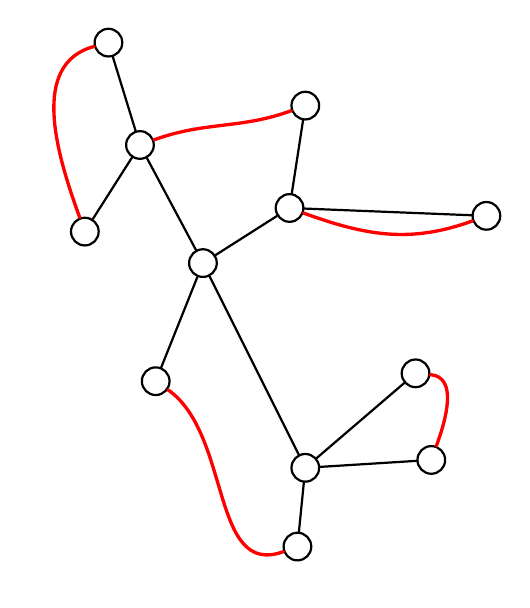
\begin{tikzpicture}[
		every node/.style={circle, draw, thick, inner sep=0pt, minimum size=10pt},
		tree edge/.style={thick},
		match/.style={red, very thick},
		line cap=round,
		line join=round
		]
		
		% ---- вершины ----
		\node (a) at (0.0,  3.2) {};   
		\node (b) at (0.4,  1.9) {};   
		\node (c) at (-0.3, 0.8) {};   
		
		\node (d) at (2.5,  2.4) {};   
		\node (e) at (2.3,  1.1) {};   
		\node (f) at (1.2,  0.4) {};   
		
		\node (g) at (0.6, -1.1) {};   
		\node (h) at (2.5, -2.2) {};   
		\node (i) at (3.9, -1.0) {};   
		\node (j) at (4.1, -2.1) {}; 
		\node (k) at (2.4, -3.2) {};  
		\node (r) at (4.8,  1.0) {};   
		
		% ---- рёбра дерева ----
		\draw[tree edge] (a)--(b);
		\draw[tree edge] (b)--(c);
		\draw[tree edge] (b)--(f);
		
		\draw[tree edge] (f)--(e);
		\draw[tree edge] (e)--(d);
		\draw[tree edge] (e)--(r);
		
		\draw[tree edge] (f)--(g);
		\draw[tree edge] (f)--(h);
		\draw[tree edge] (h)--(i);
		\draw[tree edge] (h)--(j);
		\draw[tree edge] (h)--(k);
		
		\draw[match] (a) to[out=195,in=110] (c);
		\draw[match] (b) to[out=20,in=200] (d);
		\draw[match] (e) to[out=-20,in=200] (r);
		\draw[match] (g) to[out=-35,in=200] (k);
		\draw[match] (i) to[out=-5,in=70] (j);
	\end{tikzpicture}
}
\end{center}

\begin{Theorem}{Алгоритм Кристофидеса--Сердюкова даёт $\frac{3}{2}$-приближение}{}
	Для метрической задачи коммивояжёра алгоритм Кристофидеса--Сердюкова строит гамильтонов цикл $\widetilde{H}$ такой, что:
	\[
	c(\widetilde{H}) \leq \tfrac{3}{2}\,c(H^*).
	\]
\end{Theorem}

\begin{proof}
Вес $c(\widetilde{H})$ не превышает суммарного веса Эйлерова пути в $T'$:
\[
c(\widetilde{H}) \leq c(T) + c(M),
\]
где $c(M) = \sum_{e \in M} c(e)$ — вес минимального паросочетания на $V_0$.

\emph{Шаг 1: $c(T) \leq c(H^*)$.} Доказано выше (в любом остовном дереве).

\emph{Шаг 2: $c(M) \leq \tfrac{c(H^*)}{2}$.} Пронумеруем вершины $V_0 = \{v_1, v_2, \ldots, v_{|V_0|}\}$ в порядке их встречаемости при обходе оптимального гамильтонова цикла $H^*$. Рассмотрим два паросочетания на $V_0$:
\[
M_1 = \{v_1v_2,\; v_3v_4,\; \ldots\}, \qquad M_2 = \{v_2v_3,\; v_4v_5,\; \ldots\}.
\]
По неравенству треугольника (применяя обобщённое неравенство к путям $H^*$ между соответствующими вершинами $V_0$):
\[
c(M_1) + c(M_2) \leq c(H^*).
\]
Следовательно, $\min(c(M_1),c(M_2)) \leq \tfrac{c(H^*)}{2}$. Минимальное паросочетание на $V_0$ не хуже наилучшего из $M_1,M_2$:
\[
c(M) \leq \min(c(M_1),c(M_2)) \leq \tfrac{c(H^*)}{2}.
\]

\emph{Итог:}
\[
c(\widetilde{H}) \leq c(T) + c(M) \leq c(H^*) + \tfrac{c(H^*)}{2} = \tfrac{3}{2}\,c(H^*).
\]
\end{proof}

Ключевую идею оценки минимального паросочетания на $V_0$ иллюстрирует следующая схема: цикл $H^*$ разбивается на два паросочетания $M_1$ (синие рёбра) и $M_2$ (зелёные рёбра), и их суммарный вес не превосходит $c(H^*)$.

\begin{center}
	\begin{tikzpicture}[
		dot/.style={
			circle, draw, fill=white, thick,
			inner sep=0pt, minimum size=7pt
		},
		m1/.style={thmFrame, very thick},
		m2/.style={exFrame, very thick},
		vlabel/.style={draw=none, fill=none, font=\small},
		cap/.style={draw=none, fill=none, font=\small, align=center, text width=3.6cm}
		]
		
		% --------- макрос для более выпуклого "облака" ----------
		\newcommand{\cloudcycle}[4]{%
			\draw[thick]
			(#1) .. controls ($(#1)+(-0.15,0.65)$) and ($(#2)+(-0.45,0.35)$) .. (#2)
			.. controls ($(#2)+(0.45,0.35)$) and ($(#3)+(0.15,0.55)$) .. (#3)
			.. controls ($(#3)+(0.10,-0.45)$) and ($(#4)+(0.55,0.10)$) .. (#4)
			.. controls ($(#4)+(-0.45,-0.55)$) and ($(#1)+(0.00,-0.55)$) .. (#1);
		}
		
		% =======================================================
		% Рисунок 1
		% =======================================================
		\begin{scope}[xshift=0cm]
			\node[dot] (A1) at (0.0, 0.6) {};
			\node[vlabel, above left=1pt and 1pt] at (A1) {$v_1$};
			
			\node[dot] (A2) at (1.25, 1.05) {};
			\node[vlabel, above=1pt] at (A2) {$v_2$};
			
			\node[dot] (A3) at (2.45, 0.48) {};
			\node[vlabel, above right=1pt and 1pt] at (A3) {$v_3$};
			
			\node[dot] (A4) at (1.25, -0.42) {};
			\node[vlabel, below=1pt] at (A4) {$v_4$};
			
			\cloudcycle{A1}{A2}{A3}{A4}
			
			\node[cap] at (1.25, -1.25) {$H^*$, $V_0=\{v_1,v_2,v_3,v_4\}$};
		\end{scope}
		
		% =======================================================
		% Рисунок 2
		% =======================================================
		\begin{scope}[xshift=4.9cm]
			\node[dot] (B1) at (0.0, 0.6) {};
			\node[vlabel, above left=1pt and 1pt] at (B1) {$v_1$};
			
			\node[dot] (B2) at (1.25, 1.05) {};
			\node[vlabel, above=1pt] at (B2) {$v_2$};
			
			\node[dot] (B3) at (2.45, 0.48) {};
			\node[vlabel, above right=1pt and 1pt] at (B3) {$v_3$};
			
			\node[dot] (B4) at (1.25, -0.42) {};
			\node[vlabel, below=1pt] at (B4) {$v_4$};
			
			\cloudcycle{B1}{B2}{B3}{B4}
			
			\draw[m1] (B1)--(B2);
			\draw[m1] (B3)--(B4);
			
			\node[cap, text=thmFrame] at (1.25, -1.25)
			{$M_1=\{v_1v_2,\;v_3v_4\}$};
		\end{scope}
		
		% =======================================================
		% Рисунок 3
		% =======================================================
		\begin{scope}[xshift=9.8cm]
			\node[dot] (C1) at (0.0, 0.6) {};
			\node[vlabel, above left=1pt and 1pt] at (C1) {$v_1$};
			
			\node[dot] (C2) at (1.25, 1.05) {};
			\node[vlabel, above=1pt] at (C2) {$v_2$};
			
			\node[dot] (C3) at (2.45, 0.48) {};
			\node[vlabel, above right=1pt and 1pt] at (C3) {$v_3$};
			
			\node[dot] (C4) at (1.25, -0.42) {};
			\node[vlabel, below=1pt] at (C4) {$v_4$};
			
			\cloudcycle{C1}{C2}{C3}{C4}
			
			\draw[m2] (C2)--(C3);
			\draw[m2] (C4)--(C1);
			
			\node[cap, text=exFrame] at (1.25, -1.25)
			{$M_2=\{v_2v_3,\;v_4v_1\}$};
		\end{scope}
		
	\end{tikzpicture}
\end{center}

\begin{Remark}{}{}
	Алгоритм Кристофидеса--Сердюкова долгое время оставался лучшим известным приближением для метрического TSP. Лишь в 2020--2023 годах были получены алгоритмы с коэффициентом $\tfrac{3}{2} - \varepsilon$ для частных случаев (например, для графового TSP).
\end{Remark}